\documentclass{article}
\usepackage{ifthen}
\usepackage{epsfig}
\usepackage[utf8]{inputenc}
\usepackage{xcolor}
% Packages requested by user
\usepackage{times}
\usepackage{amsmath}
\usepackage{xr}
\usepackage{amsfonts}
\usepackage{tikz}

\usepackage{newunicodechar}
  \newunicodechar{⁻}{${}^{-}$}% Superscript minus
  \newunicodechar{²}{${}^{2}$}% Superscript two
  \newunicodechar{³}{${}^{3}$}% Superscript three

\pagestyle{empty}
\begin{document}
\[
  m = \begin{pmatrix}
     1 + 5\,i & 2+6\,i \\
     3 + 7\,i & 4+ 8\,i
  \end{pmatrix}
\]
\pagebreak

\[
  m = \begin{pmatrix}
     1 & 2 & 3 & 4 \\
     0 & 0 & 0 & 0 \\
     5 & 6 & 7 & 8 \\
     i & i & i & i
  \end{pmatrix}
\]
\pagebreak

$|x\rangle|y\rangle\dots$
\pagebreak

$\sqrt{x^2 + y^2 + \dots}$
\pagebreak

$\text{coeff} \sqrt{x^2 + y^2 + \dots}$
\pagebreak

$1/\sqrt{x^2 + y^2 + \dots}$
\pagebreak

$\text{coeff}/\sqrt{x^2 + y^2 + \dots}$
\pagebreak

$\text{coeff}/\sqrt{(x-\Delta_x)^2 + (y-\Delta_y)^2 + \dots}$
\pagebreak

$|x\rangle|y\rangle|z\rangle\dots$
\pagebreak

$x \; y \; z \dots$
\pagebreak

$\text{coeff} \; x \; y \; z \dots$
\pagebreak

$1/(x \; y \; z \dots)$
\pagebreak

$\text{coeff}/(x \; y \; z \dots)$
\pagebreak

$|x_1\rangle|x_2\rangle|y_1\rangle|y_2\rangle\dots$
\pagebreak

$\sqrt{(x_1-x_2)^2 + (y_1-y_2)^2 + \dots}$
\pagebreak

$\text{coeff}\sqrt{(x_1-x_2)^2 + (y_1-y_2)^2 + \dots}$
\pagebreak

$1/\sqrt{(x_1-x_2)^2 + (y_1-y_2)^2 + \dots}$
\pagebreak

$\text{coeff}/\sqrt{(x_1-x_2)^2 + (y_1-y_2)^2 + \dots}$
\pagebreak

$\text{coeff}/\sqrt{(x_1-x_2-\Delta_x)^2 + (y_1-y_2-\Delta_y)^2 + \dots}$
\pagebreak

$\text{coeff}/\sqrt{f_x \, (x_1-x_2-\Delta_x)^2 + f_y \; (y_1-y_2-\Delta_y)^2 + \dots}$
\pagebreak

\[ 
\begin{aligned}
    |00\rangle & \rightarrow \, 0 \\
    |01\rangle & \rightarrow \, 1 \\
    |10\rangle & \rightarrow \, 2 \\
    |11\rangle & \rightarrow \, 3
\end{aligned}
\]
\pagebreak

\[ 
\begin{aligned}
    |000\rangle & \rightarrow \, 0 \\
    |001\rangle & \rightarrow \, 1 \\
    |010\rangle & \rightarrow \, 2 \\
    |011\rangle & \rightarrow \, 3 \\
    |100\rangle & \rightarrow \,-4 \\
    |101\rangle & \rightarrow \,-3 \\
    |110\rangle & \rightarrow \,-2 \\
    |111\rangle & \rightarrow \,-1
\end{aligned}
\]
\pagebreak

\[ 
     \text{qrealBytes} \times 2 \times 2^\text{numQubits}\;\;\text{(bytes)},
\]
\pagebreak

$\log_2(\text{N})$
\pagebreak

\[ 
     2 \times \text{qrealBytes} \times 2 \times 2^\text{numQubits}/N  \;\;\text{(bytes)},
\]
\pagebreak

\[ 
     \text{qrealBytes} \times 2 \times 2^{2 \times\text{numQubits}}\;\;\text{(bytes)},
\]
\pagebreak

$\log_2(\text{N})/2$
\pagebreak

\[ 
     2 \times \text{qrealBytes} \times 2 \times 2^{2\times\text{numQubits}}/N  \;\;\text{(bytes)},
\]
\pagebreak

\[
     2^{\text{numQubits}} \times 2^{\text{numQubits}},
\]
\pagebreak

\[ 
     0.31 \, X_0 \, X_2 \, Y_3 -0.2 \, Z_0 \, Y_1 \,.
\]
\pagebreak

$2^{\text{numQubits}}$
\pagebreak

$N$
\pagebreak

$2^{\text{numQubits}}/N$
\pagebreak

$\{\lambda_j\}$
\pagebreak

\[
     \begin{aligned}
     \text{hamil} &= \sum\limits_j^{\text{numSumTerms}} \lambda_j
                     \bigotimes\limits_{k_j} \hat{Z}_k \\
     &\equiv \begin{pmatrix}
             r_1 \\ & r_2 \\ & & r_3 \\ & & & \ddots \\ & & & & r_{2^{\,\text{numQubits}}}
         \end{pmatrix},
     \end{aligned}
\]
\pagebreak

\[
     \text{op} \; \rightarrow \; \text{diag}
         \big( \; r_1, \; r_2, \; r_3, \; \dots, \; r_{2^{\,\text{numQubits}}} \, \big),
\]
\pagebreak

\[
      r_i = \sum\limits_j \, s_{ij} \, \lambda_j, \;\;\;\; s_{ij} = \pm  1 \,.
\]
\pagebreak

$d_j = \text{op.real}[j] + (\text{op.imag}[j])\,\text{i} $
\pagebreak

\[
 \hat{D} = \begin{pmatrix}
 d_0 \\
 & d_1 \\
 & & \ddots \\
 & & & d_{2^{\text{op.numQubits}}-1}
 \end{pmatrix}.
\]
\pagebreak

$|\psi\rangle$
\pagebreak

$|\psi\rangle \rightarrow \hat{D} \, |\psi\rangle$
\pagebreak

$\rho$
\pagebreak

$\rho \rightarrow \hat{D}\, \rho$
\pagebreak

$\hat{D}$
\pagebreak

$ D $
\pagebreak

$ d_i $
\pagebreak

$|\psi\rangle $
\pagebreak

\[
 \langle \psi | D | \psi \rangle = \sum_i |\psi_i|^2 \, d_i
\]
\pagebreak

$ \rho $
\pagebreak

\[ 
 \text{Trace}( D \rho ) = \sum_i \rho_{ii} \, d_i
\]
\pagebreak

\[
  \hat{D} = 
  \begin{pmatrix}
  d_1 & & & \\
  & d_2 & & \\
  & & d_3 & \\
  & & & \ddots
  \end{pmatrix}
  \]
\pagebreak

$|d_i|=1 \; \forall \; i$
\pagebreak

\[
       |\psi\rangle \rightarrow \hat{D}_{\text{targets}} |\psi\rangle
  \]
\pagebreak

\[
       \rho \rightarrow \hat{D}_{\text{targets}} \; \rho \; \hat{D}_{\text{targets}}^\dagger
  \]
\pagebreak

\[
            \begin{tikzpicture}[scale=.5]
            \node[draw=none] at (-3.5, 1) {targets};

            \draw (-2,0) -- (-1, 0);
            \draw (1, 0) -- (2, 0);
            \draw (-2,2) -- (-1, 2);
            \draw (1, 2) -- (2, 2);
            \draw (-1,-1)--(-1,3)--(1,3)--(1,-1);
            \node[draw=none] at (0, 1) {$\hat{D}$};
            \node[draw=none] at (0, -1) {$\vdots$};
            
            \end{tikzpicture}
\]
\pagebreak

\[
     |\psi\rangle \rightarrow \hat{D}_{\text{targets}} |\psi\rangle
\]
\pagebreak

\[
     \rho \rightarrow \hat{D}_{\text{targets}} \; \rho
\]
\pagebreak

$ {| 0 \rangle}^{\otimes N} $
\pagebreak

$ N $
\pagebreak

$ {| 0 \rangle\langle 0 |}^{\otimes N} $
\pagebreak

\[ 
  {| + \rangle}^{\otimes N} = \frac{1}{\sqrt{2^N}} (| 0 \rangle + | 1 \rangle)^{\otimes N}\,.
\]
\pagebreak

\[ 
  {| + \rangle\langle+|}^{\otimes N} = \frac{1}{{2^N}} \sum_i\sum_j |i\rangle\langle j|\,.
\]
\pagebreak

$ | \text{stateInd} \rangle $
\pagebreak

$ | \text{stateInd} \rangle \langle \text{stateInd} | $
\pagebreak

$ | 00 \dots 00 \rangle $
\pagebreak

$ | 00 \dots 01 \rangle $
\pagebreak

$ 2^N - 1 $
\pagebreak

$ | 11 \dots 11 \rangle $
\pagebreak

$n$
\pagebreak

$2n/10 + i(2n+1)/10$
\pagebreak

$ |0\rangle $
\pagebreak

$ |1\rangle $
\pagebreak

$\theta$
\pagebreak

\[
\begin{pmatrix}
1 & 0 \\
0 & \exp(i \theta)
\end{pmatrix}
\]
\pagebreak

\[
             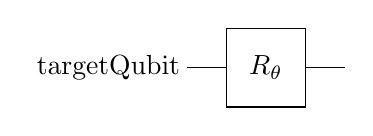
\begin{tikzpicture}[scale=.5]
             \node[draw=none] at (-4, 0) {targetQubit};

             \draw (-2,0) -- (-1, 0);
             \draw (1, 0) -- (2, 0);
             \draw (-1,-1)--(-1,1)--(1,1)--(1,-1)--cycle;
             \node[draw=none] at (0, 0) {$R_\theta$};
             \end{tikzpicture}
 \]
\pagebreak

$ \exp(i \theta) $
\pagebreak

$ |11\rangle $
\pagebreak

\[
\begin{pmatrix}
1 & & & \\
& 1 & & \\
& & 1 & \\
& & & \exp(i \theta)
\end{pmatrix}
\]
\pagebreak

\[
             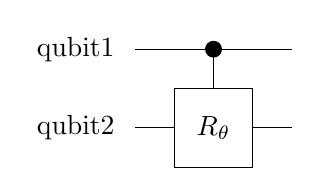
\begin{tikzpicture}[scale=.5]
             \node[draw=none] at (-3.5, 2) {qubit1};
             \node[draw=none] at (-3.5, 0) {qubit2};

             \draw (-2, 2) -- (2, 2);
             \draw[fill=black] (0, 2) circle (.2);
             \draw (0, 2) -- (0, 1);
             
             \draw (-2,0) -- (-1, 0);
             \draw (1, 0) -- (2, 0);
             \draw (-1,-1)--(-1,1)--(1,1)--(1,-1)--cycle;
             \node[draw=none] at (0, 0) {$R_\theta$};
             \end{tikzpicture}
 \]
\pagebreak

$ |1 \dots 1 \rangle $
\pagebreak

\[
             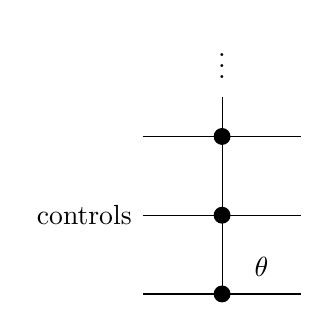
\begin{tikzpicture}[scale=.5]
             \node[draw=none] at (-3.5, 2) {controls};
             \node[draw=none] at (1, .7) {$\theta$};
             
             \node[draw=none] at (0, 6) {$\vdots$};
             \draw (0, 5) -- (0, 4);
             
             \draw (-2, 4) -- (2, 4);
             \draw[fill=black] (0, 4) circle (.2);
             \draw (0, 4) -- (0, 2); 
             
             \draw (-2, 2) -- (2, 2);
             \draw[fill=black] (0, 2) circle (.2);
             \draw (0, 2) -- (0, 0);
             
             \draw (-2,0) -- (2, 0);
             \draw[fill=black] (0, 0) circle (.2);
             \end{tikzpicture}
\]
\pagebreak

\[
\begin{pmatrix}
1 \\
& 1 \\\
& & 1 \\
& & & -1 
\end{pmatrix}
\]
\pagebreak

\[
             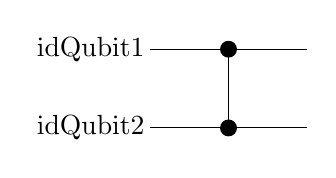
\begin{tikzpicture}[scale=.5]
             \node[draw=none] at (-3.5, 2) {idQubit1};
             \node[draw=none] at (-3.5, 0) {idQubit2};

             \draw (-2, 2) -- (2, 2);
             \draw[fill=black] (0, 2) circle (.2);
             \draw (0, 2) -- (0, 0);
             
             \draw (-2,0) -- (2, 0);
             \draw[fill=black] (0, 0) circle (.2);
             \end{tikzpicture}
 \]
\pagebreak

\[
\begin{pmatrix}
1 \\
& 1 \\\
& & \ddots \\
& & & 1 \\
& & & & -1 
\end{pmatrix}
\]
\pagebreak

\[
             \begin{tikzpicture}[scale=.5]
             \node[draw=none] at (-3.5, 2) {controls};
             
             \node[draw=none] at (0, 6) {$\vdots$};
             \draw (0, 5) -- (0, 4);
             
             \draw (-2, 4) -- (2, 4);
             \draw[fill=black] (0, 4) circle (.2);
             \draw (0, 4) -- (0, 2); 
             
             \draw (-2, 2) -- (2, 2);
             \draw[fill=black] (0, 2) circle (.2);
             \draw (0, 2) -- (0, 0);
             
             \draw (-2,0) -- (2, 0);
             \draw[fill=black] (0, 0) circle (.2);
             \end{tikzpicture}
\]
\pagebreak

$\pi/2$
\pagebreak

\[
\begin{pmatrix}
1 & 0 \\
0 & i
\end{pmatrix}
\]
\pagebreak

\[
             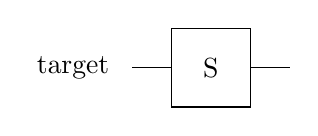
\begin{tikzpicture}[scale=.5]
             \node[draw=none] at (-3.5, 0) {target};

             \draw (-2,0) -- (-1, 0);
             \draw (1, 0) -- (2, 0);
             \draw (-1,-1)--(-1,1)--(1,1)--(1,-1)--cycle;
             \node[draw=none] at (0, 0) {S};
             \end{tikzpicture}
 \]
\pagebreak

$\pi/4$
\pagebreak

\[
\begin{pmatrix}
1 & 0 \\
0 & \exp\left(i \frac{\pi}{4}\right)
\end{pmatrix}
\]
\pagebreak

\[
             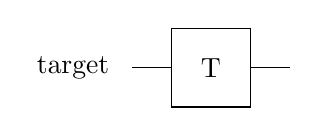
\begin{tikzpicture}[scale=.5]
             \node[draw=none] at (-3.5, 0) {target};

             \draw (-2,0) -- (-1, 0);
             \draw (1, 0) -- (2, 0);
             \draw (-1,-1)--(-1,1)--(1,1)--(1,-1)--cycle;
             \node[draw=none] at (0, 0) {T};
             \end{tikzpicture}
 \]
\pagebreak

$2^{N}$
\pagebreak

$N = $
\pagebreak

$ \psi $
\pagebreak

\[
     \sum\limits_i |\psi_i|^2
\]
\pagebreak

\[
     \text{Trace}(\rho) = \sum\limits_i \rho_{i,i} \;
\]
\pagebreak

$\alpha$
\pagebreak

$\beta$
\pagebreak

\[
U =
\begin{pmatrix}
\alpha & -\beta^* \\
\beta & \alpha^*
\end{pmatrix}
\]
\pagebreak

$|\alpha|^2 + |\beta|^2 = 1$
\pagebreak

\[
             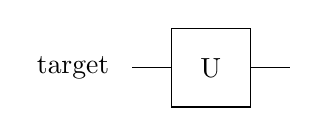
\begin{tikzpicture}[scale=.5]
             \node[draw=none] at (-3.5, 0) {target};

             \draw (-2,0) -- (-1, 0);
             \draw (1, 0) -- (2, 0);
             \draw (-1,-1)--(-1,1)--(1,1)--(1,-1)--cycle;
             \node[draw=none] at (0, 0) {U};
             \end{tikzpicture}
 \]
\pagebreak

$ u \, |\text{qureg}\rangle $
\pagebreak

$ u \, \rho \, u^\dagger $
\pagebreak

\[
\begin{pmatrix}
\cos\theta/2 & -i \sin \theta/2\\
-i \sin \theta/2 & \cos \theta/2
\end{pmatrix}
\]
\pagebreak

\[
             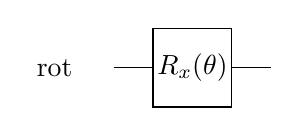
\begin{tikzpicture}[scale=.5]
             \node[draw=none] at (-3.5, 0) {rot};

             \draw (-2,0) -- (-1, 0);
             \draw (1, 0) -- (2, 0);
             \draw (-1,-1)--(-1,1)--(1,1)--(1,-1)--cycle;
             \node[draw=none] at (0, 0) {$R_x(\theta)$};
             \end{tikzpicture}
 \]
\pagebreak

\[
\begin{pmatrix}
\cos\theta/2 & - \sin \theta/2\\
\sin \theta/2 & \cos \theta/2
\end{pmatrix}
\]
\pagebreak

\[
             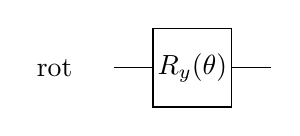
\begin{tikzpicture}[scale=.5]
             \node[draw=none] at (-3.5, 0) {rot};

             \draw (-2,0) -- (-1, 0);
             \draw (1, 0) -- (2, 0);
             \draw (-1,-1)--(-1,1)--(1,1)--(1,-1)--cycle;
             \node[draw=none] at (0, 0) {$R_y(\theta)$};
             \end{tikzpicture}
 \]
\pagebreak

\[
\begin{pmatrix}
\exp(-i \theta/2) & 0 \\
0 & \exp(i \theta/2)
\end{pmatrix}
\]
\pagebreak

\[
             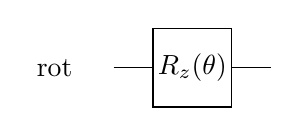
\begin{tikzpicture}[scale=.5]
             \node[draw=none] at (-3.5, 0) {rot};

             \draw (-2,0) -- (-1, 0);
             \draw (1, 0) -- (2, 0);
             \draw (-1,-1)--(-1,1)--(1,1)--(1,-1)--cycle;
             \node[draw=none] at (0, 0) {$R_z(\theta)$};
             \end{tikzpicture}
 \]
\pagebreak

$\vec{n}$
\pagebreak

$R_{\hat{n}} = \exp \left(- i \frac{\theta}{2} \hat{n} \cdot \vec{\sigma} \right) $
\pagebreak

$\vec{\sigma}$
\pagebreak

\[
             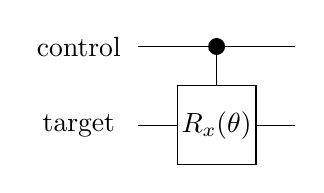
\begin{tikzpicture}[scale=.5]
             \node[draw=none] at (-3.5, 2) {control};
             \node[draw=none] at (-3.5, 0) {target};

             \draw (-2, 2) -- (2, 2);
             \draw[fill=black] (0, 2) circle (.2);
             \draw (0, 2) -- (0, 1);
             
             \draw (-2,0) -- (-1, 0);
             \draw (1, 0) -- (2, 0);
             \draw (-1,-1)--(-1,1)--(1,1)--(1,-1)--cycle;
             \node[draw=none] at (0, 0) {$R_x(\theta)$};
             \end{tikzpicture}
 \]
\pagebreak

\[
             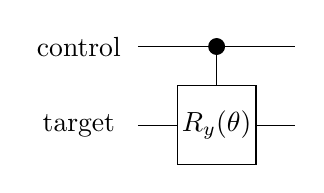
\begin{tikzpicture}[scale=.5]
             \node[draw=none] at (-3.5, 2) {control};
             \node[draw=none] at (-3.5, 0) {target};

             \draw (-2, 2) -- (2, 2);
             \draw[fill=black] (0, 2) circle (.2);
             \draw (0, 2) -- (0, 1);
             
             \draw (-2,0) -- (-1, 0);
             \draw (1, 0) -- (2, 0);
             \draw (-1,-1)--(-1,1)--(1,1)--(1,-1)--cycle;
             \node[draw=none] at (0, 0) {$R_y(\theta)$};
             \end{tikzpicture}
 \]
\pagebreak

\[
             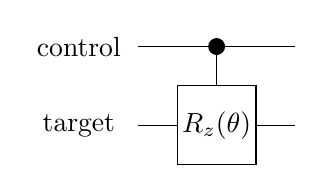
\begin{tikzpicture}[scale=.5]
             \node[draw=none] at (-3.5, 2) {control};
             \node[draw=none] at (-3.5, 0) {target};

             \draw (-2, 2) -- (2, 2);
             \draw[fill=black] (0, 2) circle (.2);
             \draw (0, 2) -- (0, 1);
             
             \draw (-2,0) -- (-1, 0);
             \draw (1, 0) -- (2, 0);
             \draw (-1,-1)--(-1,1)--(1,1)--(1,-1)--cycle;
             \node[draw=none] at (0, 0) {$R_z(\theta)$};
             \end{tikzpicture}
 \]
\pagebreak

\[
             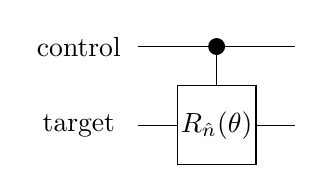
\begin{tikzpicture}[scale=.5]
             \node[draw=none] at (-3.5, 2) {control};
             \node[draw=none] at (-3.5, 0) {target};

             \draw (-2, 2) -- (2, 2);
             \draw[fill=black] (0, 2) circle (.2);
             \draw (0, 2) -- (0, 1);
             
             \draw (-2,0) -- (-1, 0);
             \draw (1, 0) -- (2, 0);
             \draw (-1,-1)--(-1,1)--(1,1)--(1,-1)--cycle;
             \node[draw=none] at (0, 0) {$R_{\hat{n}}(\theta)$};
             \end{tikzpicture}
 \]
\pagebreak

\[
\begin{pmatrix}
1 \\
& 1 \\
& & \alpha & -\beta^* \\
& & \beta & \alpha^*
\end{pmatrix}
\]
\pagebreak

\[
             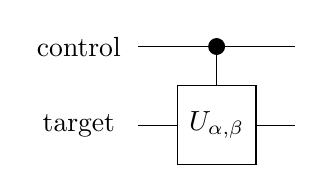
\begin{tikzpicture}[scale=.5]
             \node[draw=none] at (-3.5, 2) {control};
             \node[draw=none] at (-3.5, 0) {target};

             \draw (-2, 2) -- (2, 2);
             \draw[fill=black] (0, 2) circle (.2);
             \draw (0, 2) -- (0, 1);
             
             \draw (-2,0) -- (-1, 0);
             \draw (1, 0) -- (2, 0);
             \draw (-1,-1)--(-1,1)--(1,1)--(1,-1)--cycle;
             \node[draw=none] at (0, 0) {$U_{\alpha, \beta}$};
             \end{tikzpicture}
 \]
\pagebreak

\[
\begin{pmatrix}
1 \\
& 1 \\
& & u_{00} & u_{01}\\
& & u_{10} & u_{11}
\end{pmatrix}
\]
\pagebreak

\[
             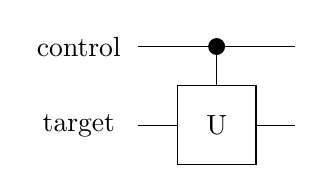
\begin{tikzpicture}[scale=.5]
             \node[draw=none] at (-3.5, 2) {control};
             \node[draw=none] at (-3.5, 0) {target};

             \draw (-2, 2) -- (2, 2);
             \draw[fill=black] (0, 2) circle (.2);
             \draw (0, 2) -- (0, 1);
             
             \draw (-2,0) -- (-1, 0);
             \draw (1, 0) -- (2, 0);
             \draw (-1,-1)--(-1,1)--(1,1)--(1,-1)--cycle;
             \node[draw=none] at (0, 0) {U};
             \end{tikzpicture}
 \]
\pagebreak

\[
\begin{pmatrix}
1 \\
& 1 \\\
& & \ddots \\
& & & u_{00} & u_{01}\\
& & & u_{10} & u_{11}
\end{pmatrix}
\]
\pagebreak

\[
             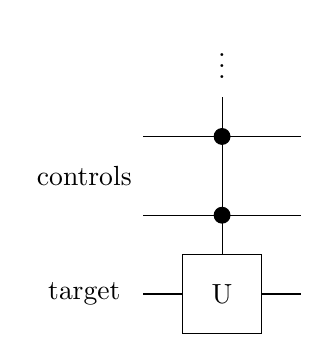
\begin{tikzpicture}[scale=.5]
             \node[draw=none] at (-3.5, 3) {controls};
             \node[draw=none] at (-3.5, 0) {target};

             \node[draw=none] at (0, 6) {$\vdots$};
             \draw (0, 5) -- (0, 4);
             
             \draw (-2, 4) -- (2, 4);
             \draw[fill=black] (0, 4) circle (.2);
             \draw (0, 4) -- (0, 2);         
             
             \draw (-2, 2) -- (2, 2);
             \draw[fill=black] (0, 2) circle (.2);
             \draw (0, 2) -- (0, 1);
             
             \draw (-2,0) -- (-1, 0);
             \draw (1, 0) -- (2, 0);
             \draw (-1,-1)--(-1,1)--(1,1)--(1,-1)--cycle;
             \node[draw=none] at (0, 0) {U};
             \end{tikzpicture}
 \]
\pagebreak

$\pi$
\pagebreak

\[
\begin{pmatrix}
0 & 1 \\
1 & 0
\end{pmatrix}
\]
\pagebreak

\[
             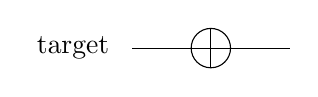
\begin{tikzpicture}[scale=.5]
             \node[draw=none] at (-3.5, 0) {target};

             \draw (-2,0) -- (2, 0);
             \draw (0, 0) circle (.5);
             \draw (0, .5) -- (0, -.5);
             \end{tikzpicture}
 \]
\pagebreak

\[
\begin{pmatrix}
0 & -i \\
i & 0
\end{pmatrix}
\]
\pagebreak

\[
             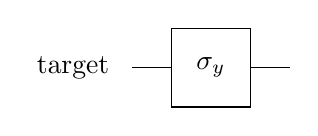
\begin{tikzpicture}[scale=.5]
             \node[draw=none] at (-3.5, 0) {target};

             \draw (-2,0) -- (-1, 0);
             \draw (1, 0) -- (2, 0);
             \draw (-1,-1)--(-1,1)--(1,1)--(1,-1)--cycle;
             \node[draw=none] at (0, 0) {$\sigma_y$};
             \end{tikzpicture}
 \]
\pagebreak

\[
\begin{pmatrix}
1 & 0 \\
0 & -1
\end{pmatrix}
\]
\pagebreak

\[
             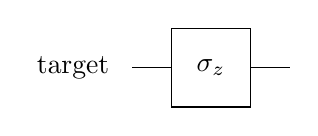
\begin{tikzpicture}[scale=.5]
             \node[draw=none] at (-3.5, 0) {target};

             \draw (-2,0) -- (-1, 0);
             \draw (1, 0) -- (2, 0);
             \draw (-1,-1)--(-1,1)--(1,1)--(1,-1)--cycle;
             \node[draw=none] at (0, 0) {$\sigma_z$};
             \end{tikzpicture}
 \]
\pagebreak

$|0\rangle$
\pagebreak

$|+\rangle$
\pagebreak

$|1\rangle$
\pagebreak

$|-\rangle$
\pagebreak

\[
\frac{1}{\sqrt{2}}
\begin{pmatrix}
1 & 1 \\
1 & -1
\end{pmatrix}
\]
\pagebreak

\[
             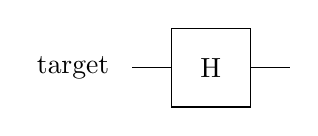
\begin{tikzpicture}[scale=.5]
             \node[draw=none] at (-3.5, 0) {target};

             \draw (-2,0) -- (-1, 0);
             \draw (1, 0) -- (2, 0);
             \draw (-1,-1)--(-1,1)--(1,1)--(1,-1)--cycle;
             \node[draw=none] at (0, 0) {H};
             \end{tikzpicture}
 \]
\pagebreak

\[
\begin{pmatrix}
1 \\
& 1 \\\
& & & 1 \\
& & 1
\end{pmatrix}
\]
\pagebreak

\[
             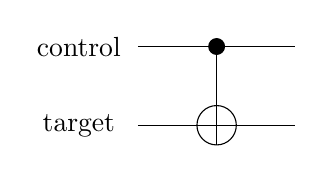
\begin{tikzpicture}[scale=.5]
             \node[draw=none] at (-3.5, 2) {control};
             \node[draw=none] at (-3.5, 0) {target};

             \draw (-2, 2) -- (2, 2);
             \draw[fill=black] (0, 2) circle (.2);
             \draw (0, 2) -- (0, -.5);
             
             \draw (-2,0) -- (2, 0);
             \draw (0, 0) circle (.5);
             \end{tikzpicture}
 \]
\pagebreak

\[
    C_{a, \,b, \,\dots}( X_c \otimes X_d \otimes \dots ) \equiv
    C_{a, \,b, \,\dots}( X_c) \; \otimes \; C_{a, \,b, \,\dots}(X_d) \; \otimes \; \dots
\]
\pagebreak

\[
\begin{pmatrix}
1 \\
& 1 \\\
& & \ddots \\
& & & &   &    & {{\scriptstyle\cdot}^{{\scriptstyle\cdot}^{{\scriptstyle\cdot}}}} \\
& & & &   & 1  &   \\
& & & & 1 &    &  \\
& & & {{\scriptstyle\cdot}^{{\scriptstyle\cdot}^{{\scriptstyle\cdot}}}} & & &
\end{pmatrix}
\]
\pagebreak

\[
             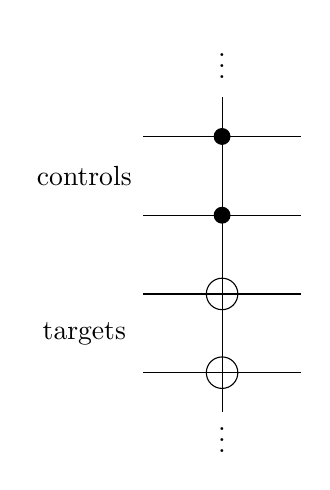
\begin{tikzpicture}[scale=.5]
             \node[draw=none] at (-3.5, 1) {targets};
             \node[draw=none] at (-3.5, 5) {controls};
             
             \node[draw=none] at (0, 8) {$\vdots$};
             \draw (0, 7) -- (0, 6);
             
             \draw (-2, 6) -- (2, 6);
             \draw[fill=black] (0, 6) circle (.2);
             \draw (0, 6) -- (0, 4);         
             
             \draw (-2, 4) -- (2, 4);
             \draw[fill=black] (0, 4) circle (.2);
             \draw(0, 4) -- (0, -1);
             
             \draw (-2,2) -- (2, 2);
             \draw (0, 2) circle (.4);

             \draw (-2,0) -- (2, 0);
             \draw (0, 0) circle (.4);
             
             \node[draw=none] at (0, -1.5) {$\vdots$};
             \end{tikzpicture}
 \]
\pagebreak

\[
    X_a \otimes X_b \otimes \dots 
\]
\pagebreak

\[
\begin{pmatrix}
 &   &    & {{\scriptstyle\cdot}^{{\scriptstyle\cdot}^{{\scriptstyle\cdot}}}} \\
 &   & 1  &   \\
 & 1 &    &  \\
 {{\scriptstyle\cdot}^{{\scriptstyle\cdot}^{{\scriptstyle\cdot}}}} & & &
\end{pmatrix}
\]
\pagebreak

\[
             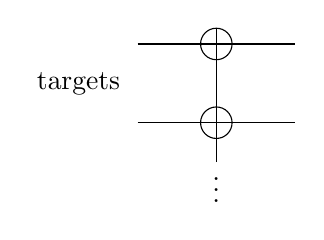
\begin{tikzpicture}[scale=.5]
             \node[draw=none] at (-3.5, 1) {targets};
             \draw (0, -1) -- (0, 2.4);
             
             \draw (-2,2) -- (2, 2);
             \draw (0, 2) circle (.4);

             \draw (-2,0) -- (2, 0);
             \draw (0, 0) circle (.4);
             
             \node[draw=none] at (0, -1.5) {$\vdots$};
             \end{tikzpicture}
 \]
\pagebreak

\[
\begin{pmatrix}
1 \\
& 1 \\\
& & & -i \\
& & i
\end{pmatrix}
\]
\pagebreak

\[
             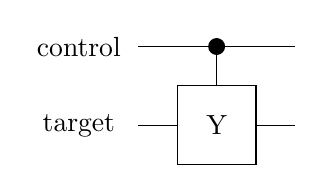
\begin{tikzpicture}[scale=.5]
             \node[draw=none] at (-3.5, 2) {control};
             \node[draw=none] at (-3.5, 0) {target};

             \draw (-2, 2) -- (2, 2);
             \draw[fill=black] (0, 2) circle (.2);
             \draw (0, 2) -- (0, 1);
             
             \draw (-2,0) -- (-1, 0);
             \draw (1, 0) -- (2, 0);
             \draw (-1,-1)--(-1,1)--(1,1)--(1,-1)--cycle;
             \node[draw=none] at (0, 0) {Y};
             \end{tikzpicture}
 \]
\pagebreak

\[
    \text{outcomeProbs} = \{ \; |\alpha_0|^2, \; |\alpha_1|^2, \; |\alpha_2|^2, \; |\alpha_3|^2, \; ... \; \},
  \]
\pagebreak

$|\alpha_j|^2$
\pagebreak

\[
     |\dots\textbf{c\,b\,a}\rangle_i \; \; = \;\; |000\rangle,  \;\; |001\rangle \;\; |010\rangle \;\; |011\rangle, \;\; \dots
  \]
\pagebreak

\[
     |\psi\rangle = \sum\limits_i^{\text{numQubits}} \alpha_i \; |\dots\textbf{c\,b\,a}\rangle_i 
       \; \otimes \; |\phi\rangle_i,
  \]
\pagebreak

\[
     \begin{aligned}
     \rho &= \sum\limits_{i,j}^{\text{numQubits}} \; \beta_{ij} \; |\dots\textbf{c\,b\,a}\rangle_i\,\langle\dots\textbf{c\,b\,a}|_j 
           \; \otimes \; \mu_{ij} \\
          &= \sum\limits_i^{\text{numQubits}} \; |\alpha_i|^2 \;  |\dots\textbf{c\,b\,a}\rangle\langle\dots\textbf{c\,b\,a}|_i  \;\; + \, 
           \sum\limits_{i \ne j}^{\text{numQubits}} \; \beta_{ij} \; |\dots\textbf{c\,b\,a}\rangle_i\,\langle\dots\textbf{c\,b\,a}|_j 
           \; \otimes \; \mu_{ij},
      \end{aligned}
  \]
\pagebreak

$|\phi\rangle_i$
\pagebreak

$\mu_{ij}$
\pagebreak

\[
     |\psi\rangle = 
         \alpha_0 |000\rangle \;+\; \alpha_1 |001\rangle \;+\; 
         \alpha_2 |010\rangle \;+\; \alpha_3 |011\rangle \;+\;
         \alpha_4 |100\rangle \;+\; \alpha_5 |101\rangle \;+\; 
         \alpha_6 |110\rangle \;+\; \alpha_7 |111\rangle,
  \]
\pagebreak

\[
     \text{outcomeProbs} = \{ \;\; |\alpha_0|^2+|\alpha_2|^2, \;\; |\alpha_4|^2+|\alpha_6|^2, \;\;
                                |\alpha_1|^2+|\alpha_3|^2, \;\; |\alpha_5|^2+|\alpha_7|^2  \;\; \}.
  \]
\pagebreak

$ \langle \text{bra} | \text{ket} \rangle $
\pagebreak

\[ 
  \langle \text{bra} | \text{ket} \rangle = \sum_i {\text{bra}_i}^* \; \times \; \text{ket}_i 
\]
\pagebreak

\[
 ((\rho_1, \rho_2))_{HS} := \text{Tr}[ \rho_1^\dagger \rho_2 ],
\]
\pagebreak

\[
 ((\rho_1, \rho_2))_{HS} = \sum\limits_i \sum\limits_j  (\rho_1)_{ij}^* (\rho_2)_{ij}
\]
\pagebreak

\[
 ((\rho_1, \rho_2))_{HS} = ((\rho_2, \rho_1))_{HS} = \text{Tr}[\rho_1 \rho_2]
\]
\pagebreak

\[
 ((\rho_1, \rho_2))_{HS} = |\langle \text{bra} | \text{ket} \rangle|^2.
\]
\pagebreak

\[
  \text{Re}\{ \text{Tr}[ \rho_1^\dagger \rho_2 ] \} = \text{Re}\{ \text{Tr}[ \rho_2^\dagger \rho_1 ] \}.
\]
\pagebreak

$ \sigma $
\pagebreak

$ H $
\pagebreak

\[
     ((\sigma, H \rho + \rho H))_{HS} = 2 \; \text{Re} \{ ((\sigma, H \rho))_{HS} \} 
\]
\pagebreak

$ H \rho $
\pagebreak

\[
(1 - \text{prob}) \, \rho + \text{prob} \; Z_q \, \rho \, Z_q
\]
\pagebreak

\[
(1 - \text{prob}) \, \rho + \frac{\text{prob}}{3} \; \left( 
     Z_a \, \rho \, Z_a + 
     Z_b \, \rho \, Z_b + 
     Z_a Z_b \, \rho \, Z_a Z_b
\right)
\]
\pagebreak

\[
(1 - \text{prob}) \, \rho + \frac{\text{prob}}{3} \; \left( 
     X_q \, \rho \, X_q + 
     Y_q \, \rho \, Y_q + 
     Z_q \, \rho \, Z_q
\right)
\]
\pagebreak

\[
     \left( 1 - \frac{4}{3} \text{prob} \right) \rho +
     \left( \frac{4}{3} \text{prob} \right) \frac{\vec{\bf{1}}}{2}
\]
\pagebreak

$ \frac{\vec{\bf{1}}}{2} $
\pagebreak

\[
 K_0 \rho K_0^\dagger + K_1 \rho K_1^\dagger
\]
\pagebreak

$K_0$
\pagebreak

$K_1$
\pagebreak

\[
     K_0 = \begin{pmatrix} 1 & 0 \\ 0 & \sqrt{1-\text{prob}} \end{pmatrix}, \;\;
     K_1 = \begin{pmatrix} 0 & \sqrt{\text{prob}} \\ 0 & 0 \end{pmatrix}.
\]
\pagebreak

$\{ IX, IY, IZ, XI, YI, ZI, XX, XY, XZ, YX, YY, YZ, ZX, ZY, ZZ \}$
\pagebreak

$II$
\pagebreak

\[
(1 - \text{prob}) \, \rho \; + \; \frac{\text{prob}}{15} \; \left( 
     \sum \limits_{\sigma_a \in \{X_a,Y_a,Z_a,I_a\}}
     \sum \limits_{\sigma_b \in \{X_b,Y_b,Z_b,I_b\}}
     \sigma_a \sigma_b \; \rho \; \sigma_a \sigma_b
\right)
- \frac{\text{prob}}{15} I_a I_b \; \rho \; I_a I_b
\]
\pagebreak

\[
(1 - \text{prob}) \, \rho + \frac{\text{prob}}{15} \; \left( 
\begin{aligned}
     &X_a \, \rho \, X_a + 
     X_b \, \rho \, X_b + 
     Y_a \, \rho \, Y_a + 
     Y_b \, \rho \, Y_b + 
     Z_a \, \rho \, Z_a + 
     Z_b \, \rho \, Z_b 
  \\
   + &X_a X_b \, \rho \, X_a X_b +
     X_a Y_b \, \rho \, X_a Y_b +
     X_a Z_b \, \rho \, X_a Z_b +
     Y_a X_b \, \rho \, Y_a X_b
\\
  + &Y_a Y_b \, \rho \, Y_a Y_b +
     Y_a Z_b \, \rho \, Y_a Z_b +
     Z_a X_b \, \rho \, Z_a X_b + 
     Z_a Y_b \, \rho \, Z_a Y_b + 
     Z_a Z_b \, \rho \, Z_a Z_b
\end{aligned}
\right)
\]
\pagebreak

\[ 
     \left( 1 - \frac{16}{15} \text{prob} \right) \rho + \left( \frac{16}{15} \text{prob} \right) \frac{\vec{\bf{1}}}{2}
\]
\pagebreak

\[
(1 - \text{probX} - \text{probY} - \text{probZ}) \, \rho + \;\;\;
     (\text{probX})\; X_q \, \rho \, X_q + \;\;\;
     (\text{probY})\; Y_q \, \rho \, Y_q + \;\;\;
     (\text{probZ})\; Z_q \, \rho \, Z_q
\]
\pagebreak

$\text{Tr}(\rho^2)$
\pagebreak

$\sum_{ij} |\rho_{ij}|^2 $
\pagebreak

\[ 
 |\langle \text{qureg} | \text{pureState} \rangle|^2
\]
\pagebreak

\[ 
 \langle \text{pureState} | \text{qureg} | \text{pureState} \rangle
\]
\pagebreak

\[
\begin{pmatrix}
1 \\
& & 1 \\\
&  1 \\
& & & 1
\end{pmatrix}
\]
\pagebreak

\[
            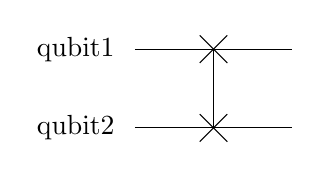
\begin{tikzpicture}[scale=.5]
            \node[draw=none] at (-3.5, 2) {qubit1};
            \node[draw=none] at (-3.5, 0) {qubit2};

            \draw (-2, 2) -- (2, 2);
            \draw (0, 2) -- (0, 0);
            \draw (-2,0) -- (2, 0);

            \draw (-.35,-.35) -- (.35,.35);
            \draw (-.35,.35) -- (.35,-.35);

            \draw (-.35,-.35 + 2) -- (.35,.35 + 2);
            \draw (-.35,.35 + 2) -- (.35,-.35 + 2);

            \end{tikzpicture}
\]
\pagebreak

\[
\begin{pmatrix}
1 \\
& \frac{1}{2}(1+i) & \frac{1}{2}(1-i) \\\
& \frac{1}{2}(1-i) & \frac{1}{2}(1+i) \\
& & & 1
\end{pmatrix}
\]
\pagebreak

\[
            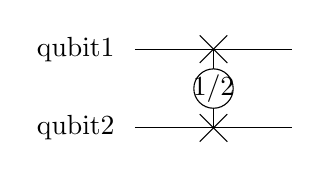
\begin{tikzpicture}[scale=.5]
            \node[draw=none] at (-3.5, 2) {qubit1};
            \node[draw=none] at (-3.5, 0) {qubit2};

            \draw (-2, 2) -- (2, 2);
            \draw (0, 2) -- (0, 0);
            \draw (-2,0) -- (2, 0);

            \draw (-.35,-.35) -- (.35,.35);
            \draw (-.35,.35) -- (.35,-.35);

            \draw (-.35,-.35 + 2) -- (.35,.35 + 2);
            \draw (-.35,.35 + 2) -- (.35,-.35 + 2);
            
            \draw[fill=white] (0, 1) circle (.5);
            \node[draw=none] at (0, 1) {1/2};

            \end{tikzpicture}
\]
\pagebreak

\[
             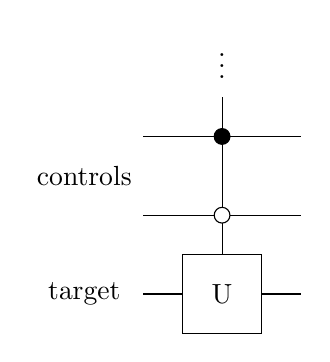
\begin{tikzpicture}[scale=.5]
             \node[draw=none] at (-3.5, 3) {controls};
             \node[draw=none] at (-3.5, 0) {target};

             \node[draw=none] at (0, 6) {$\vdots$};
             \draw (0, 5) -- (0, 4);
             
             \draw (-2, 4) -- (2, 4);
             \draw[fill=black] (0, 4) circle (.2);
             \draw (0, 4) -- (0, 2);         
             
             \draw (-2, 2) -- (2, 2);
             \draw[fill=white] (0, 2) circle (.2);
             \draw (0, 2-.2) -- (0, 1);
             
             \draw (-2,0) -- (-1, 0);
             \draw (1, 0) -- (2, 0);
             \draw (-1,-1)--(-1,1)--(1,1)--(1,-1)--cycle;
             \node[draw=none] at (0, 0) {U};
             \end{tikzpicture}
 \]
\pagebreak

\[ 
   \exp \left( - i \, \frac{\theta}{2} \; \bigotimes_{j}^{\text{numQubits}} Z_j\right)
\]
\pagebreak

$\theta =$
\pagebreak

$\exp(\pm i \theta/2)$
\pagebreak

\[ 
   \exp \left( - i \, \frac{\theta}{2} \; \bigotimes_{j}^{\text{numTargets}} \hat{\sigma}_j\right)
\]
\pagebreak

$\theta = $
\pagebreak

$\hat{\sigma}_j \in \{X, Y, Z\}$
\pagebreak

\[
   \exp \left( - i \, (0.1/2) \; X_5 \, Y_8 \, Z_9 \right) 
\]
\pagebreak

$\exp(-i \theta/2)$
\pagebreak

\[ 
   |1\rangle\langle 1|^{\otimes\, \text{numControls}} \; \otimes \,
    \exp \left( - i \, \frac{\theta}{2} \; \bigotimes_{j}^{\text{numTargets}} Z_j\right)
    \;\;+\;\; \sum\limits_{k=0}^{2^{\,\text{numControls}} - 2} |k\rangle\langle k| \otimes \text{I}
\]
\pagebreak

\[
             \begin{tikzpicture}[scale=.5]
             \node[draw=none] at (-4, 1) {targets};
             \node[draw=none] at (-4, 5) {controls};
             
             \node[draw=none] at (0, 8) {$\vdots$};
             \draw (0, 7) -- (0, 6);
             
             \draw (-2.5, 6) -- (2.5, 6);
             \draw[fill=black] (0, 6) circle (.2);
             \draw (0, 6) -- (0, 4);         
             
             \draw (-2.5, 4) -- (2.5, 4);
             \draw[fill=black] (0, 4) circle (.2);
             \draw(0, 4) -- (0, 3);

             \draw (-2.5,0) -- (-1.5, 0);
             \draw (1.5, 0) -- (2.5, 0);
             \draw (-2.5,2) -- (-1.5, 2);
             \draw (1.5, 2) -- (2.5, 2);
             \draw (-1.5,-1)--(-1.5,3)--(1.5,3)--(1.5,-1);
             \node[draw=none] at (0, 1) {$e^{-i\frac{\theta}{2}Z^{\otimes}}$};
             \node[draw=none] at (0, -1) {$\vdots$};
             
             \end{tikzpicture}
 \]
\pagebreak

\[ 
   |1\rangle\langle 1|^{\otimes\, \text{numControls}} \; \otimes \,
    \exp \left( - i \, \frac{\theta}{2} \; \bigotimes_{j}^{\text{numTargets}} \hat{\sigma}_j\right)
    \;\;+\;\; \sum\limits_{k=0}^{2^{\,\text{numControls}} - 2} |k\rangle\langle k| \otimes \text{I}
\]
\pagebreak

$\hat{\sigma}_j$
\pagebreak

\[
             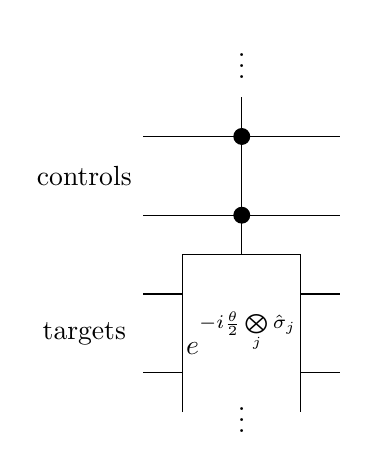
\begin{tikzpicture}[scale=.5]
             \node[draw=none] at (-4, 1) {targets};
             \node[draw=none] at (-4, 5) {controls};
             
             \node[draw=none] at (0, 8) {$\vdots$};
             \draw (0, 7) -- (0, 6);
             
             \draw (-2.5, 6) -- (2.5, 6);
             \draw[fill=black] (0, 6) circle (.2);
             \draw (0, 6) -- (0, 4);         
             
             \draw (-2.5, 4) -- (2.5, 4);
             \draw[fill=black] (0, 4) circle (.2);
             \draw(0, 4) -- (0, 3);

             \draw (-2.5,0) -- (-1.5, 0);
             \draw (1.5, 0) -- (2.5, 0);
             \draw (-2.5,2) -- (-1.5, 2);
             \draw (1.5, 2) -- (2.5, 2);
             \draw (-1.5,-1)--(-1.5,3)--(1.5,3)--(1.5,-1);
             \node[draw=none] at (0, 1) {$e^{-i\frac{\theta}{2} \bigotimes\limits_j \hat{\sigma}_j }$};
             \node[draw=none] at (0, -1) {$\vdots$};
             
             \end{tikzpicture}
 \]
\pagebreak

\[
   |1\rangle\langle 1 | \otimes \exp\left( -i \, (0.1/2) \, X_0 \, Y_1 \, Z_2 \right) \, \text{I}_3
   \;\; + \;\; |0\rangle\langle 0| \otimes \text{I}^{\otimes 4}
\]
\pagebreak

$ \sigma = \otimes_j \hat{\sigma}_j $
\pagebreak

$ \langle \psi | \sigma | \psi \rangle $
\pagebreak

$ \text{Trace}(\sigma \rho) $
\pagebreak

$ \langle \psi | I I I I X I Z | \psi \rangle $
\pagebreak

$ \sigma | \psi \rangle $
\pagebreak

$ \sigma \rho $
\pagebreak

$ \sigma^\dagger \rho \sigma $
\pagebreak

$ H = \sum_i c_i \otimes_j^{N} \hat{\sigma}_{i,j} $
\pagebreak

$ c_i \in $
\pagebreak

$ N = $
\pagebreak

$ \langle \psi | H | \psi \rangle $
\pagebreak

$ \text{Trace}(H \rho) =\text{Trace}(\rho H) $
\pagebreak

$ \langle \psi | (1.5 X I I - 3.6 X Y Z) | \psi \rangle $
\pagebreak

$ \hat{\sigma} \rho $
\pagebreak

$ \hat{\sigma} \rho \hat{\sigma}^\dagger $
\pagebreak

\[
             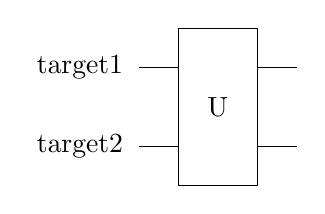
\begin{tikzpicture}[scale=.5]
             \node[draw=none] at (-3.5, 0) {target2};
             \node[draw=none] at (-3.5, 2) {target1};

             \draw (-2,0) -- (-1, 0);
             \draw (1, 0) -- (2, 0);
             \draw (-2,2) -- (-1, 2);
             \draw (1, 2) -- (2, 2);
             \draw (-1,-1)--(-1,3)--(1,3)--(1,-1)--cycle;
             \node[draw=none] at (0, 1) {U};
             \end{tikzpicture}
 \]
\pagebreak

$ |\text{targetQubit2} \;\; \text{targetQubit1}\rangle : \{ |00\rangle, |01\rangle, |10\rangle, |11\rangle \} $
\pagebreak

\[
\begin{pmatrix}
u_{00} & u_{01} & u_{02} & u_{03} \\
u_{10} & u_{11} & u_{12} & u_{13} \\
u_{20} & u_{21} & u_{22} & u_{23} \\
u_{30} & u_{31} & u_{32} & u_{33}
\end{pmatrix}
\begin{pmatrix}
|ba\rangle = |00\rangle \\
|ba\rangle = |01\rangle \\
|ba\rangle = |10\rangle \\
|ba\rangle = |11\rangle 
\end{pmatrix}
\]
\pagebreak

\[
\begin{pmatrix}
1 \\
& 1 \\
& & 1 \\
& & & 1 \\
& & & & u_{00} & u_{01} & u_{02} & u_{03} \\
& & & & u_{10} & u_{11} & u_{12} & u_{13} \\
& & & & u_{20} & u_{21} & u_{22} & u_{23} \\
& & & & u_{30} & u_{31} & u_{32} & u_{33}
\end{pmatrix}
\]
\pagebreak

\[
             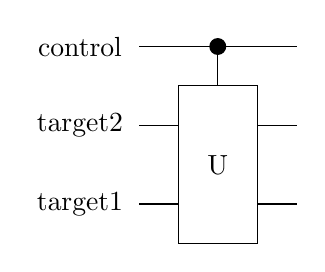
\begin{tikzpicture}[scale=.5]
             \node[draw=none] at (-3.5, 0) {target1};
             \node[draw=none] at (-3.5, 2) {target2};
             \node[draw=none] at (-3.5, 4) {control};      
             
             \draw (-2, 4) -- (2, 4);
             \draw[fill=black] (0, 4) circle (.2);
             \draw(0, 4) -- (0, 3);

             \draw (-2,0) -- (-1, 0);
             \draw (1, 0) -- (2, 0);
             \draw (-2,2) -- (-1, 2);
             \draw (1, 2) -- (2, 2);
             \draw (-1,-1)--(-1,3)--(1,3)--(1,-1)--cycle;
             \node[draw=none] at (0, 1) {U};
             \end{tikzpicture}
 \]
\pagebreak

\[
\begin{pmatrix}
1 \\
& 1 \\\
& & \ddots \\
& & & u_{00} & u_{01} & u_{02} & u_{03} \\
& & & u_{10} & u_{11} & u_{12} & u_{13} \\
& & & u_{20} & u_{21} & u_{22} & u_{23} \\
& & & u_{30} & u_{31} & u_{32} & u_{33}
\end{pmatrix}
\]
\pagebreak

\[
             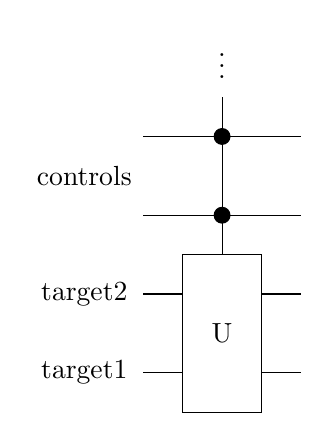
\begin{tikzpicture}[scale=.5]
             \node[draw=none] at (-3.5, 0) {target1};
             \node[draw=none] at (-3.5, 2) {target2};
             \node[draw=none] at (-3.5, 5) {controls};
             
             \node[draw=none] at (0, 8) {$\vdots$};
             \draw (0, 7) -- (0, 6);
             
             \draw (-2, 6) -- (2, 6);
             \draw[fill=black] (0, 6) circle (.2);
             \draw (0, 6) -- (0, 4);         
             
             \draw (-2, 4) -- (2, 4);
             \draw[fill=black] (0, 4) circle (.2);
             \draw(0, 4) -- (0, 3);

             \draw (-2,0) -- (-1, 0);
             \draw (1, 0) -- (2, 0);
             \draw (-2,2) -- (-1, 2);
             \draw (1, 2) -- (2, 2);
             \draw (-1,-1)--(-1,3)--(1,3)--(1,-1)--cycle;
             \node[draw=none] at (0, 1) {U};
             \end{tikzpicture}
 \]
\pagebreak

\[
\begin{pmatrix}
u_{00} & u_{01} & u_{02} & u_{03} & u_{04} & u_{05} & u_{06} & u_{07} \\
u_{10} & u_{11} & u_{12} & u_{13} & u_{14} & u_{15} & u_{16} & u_{17} \\
u_{20} & u_{21} & u_{22} & u_{23} & u_{24} & u_{25} & u_{26} & u_{27} \\
u_{30} & u_{31} & u_{32} & u_{33} & u_{34} & u_{35} & u_{36} & u_{37} \\
u_{40} & u_{41} & u_{42} & u_{43} & u_{44} & u_{45} & u_{46} & u_{47} \\
u_{50} & u_{51} & u_{52} & u_{53} & u_{54} & u_{55} & u_{56} & u_{57} \\
u_{60} & u_{61} & u_{62} & u_{63} & u_{64} & u_{65} & u_{66} & u_{67} \\
u_{70} & u_{71} & u_{72} & u_{73} & u_{74} & u_{75} & u_{76} & u_{77} \\
\end{pmatrix}
\begin{pmatrix}
|cba\rangle = |000\rangle \\
|cba\rangle = |001\rangle \\
|cba\rangle = |010\rangle \\
|cba\rangle = |011\rangle \\
|cba\rangle = |100\rangle \\
|cba\rangle = |101\rangle \\
|cba\rangle = |110\rangle \\
|cba\rangle = |111\rangle 
\end{pmatrix}
\]
\pagebreak

\[
             \begin{tikzpicture}[scale=.5]
             \node[draw=none] at (-3.5, 1) {targets};

             \draw (-2,0) -- (-1, 0);
             \draw (1, 0) -- (2, 0);
             \draw (-2,2) -- (-1, 2);
             \draw (1, 2) -- (2, 2);
             \draw (-1,-1)--(-1,3)--(1,3)--(1,-1);
             \node[draw=none] at (0, 1) {U};
             \node[draw=none] at (0, -1) {$\vdots$};
             
             \end{tikzpicture}
 \]
\pagebreak

\[
\begin{pmatrix}
1 \\
& 1 \\\
& & 1 \\
& & & 1 \\
& & & & u_{00} & u_{01} & \dots  \\
& & & & u_{10} & u_{11} & \dots \\
& & & & \vdots & \vdots & \ddots
\end{pmatrix}
\]
\pagebreak

\[
             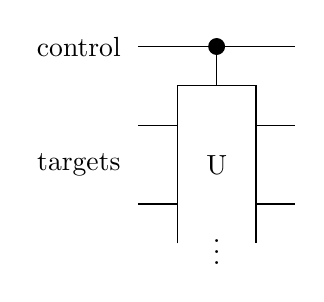
\begin{tikzpicture}[scale=.5]
             \node[draw=none] at (-3.5, 1) {targets};
             \node[draw=none] at (-3.5, 4) {control};      
             
             \draw (-2, 4) -- (2, 4);
             \draw[fill=black] (0, 4) circle (.2);
             \draw(0, 4) -- (0, 3);

             \draw (-2,0) -- (-1, 0);
             \draw (1, 0) -- (2, 0);
             \draw (-2,2) -- (-1, 2);
             \draw (1, 2) -- (2, 2);
             \draw (-1,-1)--(-1,3)--(1,3)--(1,-1);
             \node[draw=none] at (0, 1) {U};
             \node[draw=none] at (0, -1) {$\vdots$};
             
             \end{tikzpicture}
 \]
\pagebreak

\[
\begin{pmatrix}
1 \\
& 1 \\\
& & \ddots \\
& & & u_{00} & u_{01} & \dots  \\
& & & u_{10} & u_{11} & \dots \\
& & & \vdots & \vdots & \ddots
\end{pmatrix}
\]
\pagebreak

\[
             \begin{tikzpicture}[scale=.5]
             \node[draw=none] at (-3.5, 1) {targets};
             \node[draw=none] at (-3.5, 5) {controls};
             
             \node[draw=none] at (0, 8) {$\vdots$};
             \draw (0, 7) -- (0, 6);
             
             \draw (-2, 6) -- (2, 6);
             \draw[fill=black] (0, 6) circle (.2);
             \draw (0, 6) -- (0, 4);         
             
             \draw (-2, 4) -- (2, 4);
             \draw[fill=black] (0, 4) circle (.2);
             \draw(0, 4) -- (0, 3);

             \draw (-2,0) -- (-1, 0);
             \draw (1, 0) -- (2, 0);
             \draw (-2,2) -- (-1, 2);
             \draw (1, 2) -- (2, 2);
             \draw (-1,-1)--(-1,3)--(1,3)--(1,-1);
             \node[draw=none] at (0, 1) {U};
             \node[draw=none] at (0, -1) {$\vdots$};
             
             \end{tikzpicture}
 \]
\pagebreak

$K_i$
\pagebreak

\[
 \rho \to \sum\limits_i^{\text{numOps}} K_i \rho K_i^\dagger
\]
\pagebreak

$ K_i $
\pagebreak

\[
 \sum \limits_i^{\text{numOps}} K_i^\dagger K_i = I
\]
\pagebreak

$ I $
\pagebreak

\[
 D(a, b) = \| a - b \|_F = \sqrt{  \text{Tr}[ (a-b)(a-b)^\dagger ]   }
\]
\pagebreak

\[
 D(a, b) = \sqrt{ \sum\limits_i \sum\limits_j | a_{ij} - b_{ij} |^2 }
\]
\pagebreak

$ \alpha = \sum_i c_i \otimes_j^{N} \hat{\sigma}_{i,j} $
\pagebreak

$ \alpha | \psi \rangle $
\pagebreak

$ |\psi\rangle $
\pagebreak

$\alpha \rho$
\pagebreak

$ (1.5 X I I - 3.6 X Y Z) $
\pagebreak

$ \exp(-i \, \text{hamil} \, \text{time}) $
\pagebreak

$ \text{hamil} = \sum_j^N c_j \, \hat \sigma_j $
\pagebreak

$c_j$
\pagebreak

$\hat \sigma_j$
\pagebreak

\[
  \exp(-i \, \text{hamil} \, \text{time})
     \approx 
   \prod\limits^{\text{reps}} \prod\limits_{j=1}^{N} \exp(-i \, c_j \, \text{time} \, \hat\sigma_j / \text{reps})
\]
\pagebreak

\[
  \exp(-i \, \text{hamil} \, \text{time})
     \approx 
   \prod\limits^{\text{reps}} \left[
        \prod\limits_{j=1}^{N} \exp(-i \, c_j \, \text{time} \, \hat\sigma_j / (2 \, \text{reps}))
         \prod\limits_{j=N}^{1} \exp(-i \, c_j \, \text{time} \, \hat\sigma_j / (2 \, \text{reps}))
    \right]
\]
\pagebreak

$ S[\text{time}, \text{order}, \text{reps}] $
\pagebreak

\[
     S[\text{time}, \text{order}, 1] = 
         \left( \prod\limits^2 S[p \, \text{time}, \text{order}-2, 1] \right)
         S[ (1-4p)\,\text{time}, \text{order}-2, 1]
         \left( \prod\limits^2 S[p \, \text{time}, \text{order}-2, 1] \right)
\]
\pagebreak

\[
     S[\text{time}, \text{order}, \text{reps}] = 
         \prod\limits^{\text{reps}} S[\text{time}/\text{reps}, \text{order}, 1]
\]
\pagebreak

$ p = \left( 4 - 4^{1/(\text{order}-1)} \right)^{-1} $
\pagebreak

\[
\begin{pmatrix}
1 \\
& 1 \\\
& & \ddots \\
& & & m_{00} & m_{01} & \dots  \\
& & & m_{10} & m_{11} & \dots \\
& & & \vdots & \vdots & \ddots
\end{pmatrix}
\]
\pagebreak

$f(r)$
\pagebreak

\[ 
   f(r) = \sum\limits_{i}^{\text{numTerms}} \text{coeffs}[i] \; r^{\, \text{exponents}[i]}\,,
  \]
\pagebreak

\[
      f(r) =  1 \, r^2 - 3.14 \, r^{-5.5}.
  \]
\pagebreak

$r$
\pagebreak

$r=0$
\pagebreak

\[
   \alpha \, |r\rangle \rightarrow \, \exp(i f(r)) \; \alpha \, |r\rangle.
  \]
\pagebreak

\[ 
  \begin{aligned}
    |0\mathbf{00}\rangle & \rightarrow \, e^{i f(0)}\,|0\mathbf{00}\rangle \\
    |0\mathbf{01}\rangle & \rightarrow \, e^{i f(1)}\,|0\mathbf{01}\rangle \\
    |0\mathbf{10}\rangle & \rightarrow \, e^{i f(2)}\,|0\mathbf{10}\rangle \\
    |0\mathbf{11}\rangle & \rightarrow \, e^{i f(3)}\,|0\mathbf{11}\rangle \\
    |1\mathbf{00}\rangle & \rightarrow \, e^{i f(0)}\,|1\mathbf{00}\rangle \\
    |1\mathbf{01}\rangle & \rightarrow \, e^{i f(1)}\,|1\mathbf{01}\rangle \\
    |1\mathbf{10}\rangle & \rightarrow \, e^{i f(2)}\,|1\mathbf{10}\rangle \\
    |1\mathbf{11}\rangle & \rightarrow \, e^{i f(3)}\,|1\mathbf{11}\rangle
  \end{aligned}
  \]
\pagebreak

\[
     \rho \rightarrow \hat{D} \, \rho \, \hat{D}^\dagger
  \]
\pagebreak

\[
     \hat{D} = \text{diag} \, \{ \; e^{i f(r_0)}, \; e^{i f(r_1)}, \;  \dots \; \}.
  \]
\pagebreak

$\rho_{jk}$
\pagebreak

\[
     \alpha \, |j\rangle\langle k| \; \rightarrow \; e^{i (f(r_j) - f(r_k))} \; \alpha \, |j\rangle\langle k|
  \]
\pagebreak

$f(r=2)$
\pagebreak

\[ 
  \begin{aligned}
    |0\mathbf{00}\rangle & \rightarrow \, e^{i f(0)}\,|0\mathbf{00}\rangle \\
    |0\mathbf{01}\rangle & \rightarrow \, e^{i f(1)}\,|0\mathbf{01}\rangle \\
    |0\mathbf{10}\rangle & \rightarrow \, e^{i \pi} \hspace{12pt} |0\mathbf{10}\rangle \\
    |0\mathbf{11}\rangle & \rightarrow \, e^{i f(3)}\,|0\mathbf{11}\rangle \\
    |1\mathbf{00}\rangle & \rightarrow \, e^{i f(0)}\,|1\mathbf{00}\rangle \\
    |1\mathbf{01}\rangle & \rightarrow \, e^{i f(1)}\,|1\mathbf{01}\rangle \\
    |1\mathbf{10}\rangle & \rightarrow \, e^{i \pi} \hspace{12pt} |1\mathbf{10}\rangle \\
    |1\mathbf{11}\rangle & \rightarrow \, e^{i f(3)}\,|1\mathbf{11}\rangle
  \end{aligned}
  \]
\pagebreak

\[
     \rho \; \rightarrow \; \hat{D} \, \rho \hat{D}^\dagger.
  \]
\pagebreak

$f(r_j) \rightarrow \theta$
\pagebreak

$f(r_k) \rightarrow \phi$
\pagebreak

\[
     \alpha \, |j\rangle\langle k| \; \rightarrow \; 
         \exp(\, i \, (\theta - \phi) \, ) \; \alpha \, |j\rangle\langle k|.
  \]
\pagebreak

$f(\vec{r})$
\pagebreak

\[ 
   f(r_1, \; \dots, \; r_{\text{numRegs}}) = \sum\limits_j^{\text{numRegs}} \; \sum\limits_{i}^{\text{numTermsPerReg}[j]} \; c_{i,j} \; {r_j}^{\; p_{i,j}}\,,
  \]
\pagebreak

$c_{i,j}$
\pagebreak

$p_{i,j}$
\pagebreak

\[
     f(\vec{r}) =  1 \, {r_1}^2 + 2 \, {r_2} + 4 \, {r_2}^{5} - 3.14 \, {r_3}^{0.5}.
  \]
\pagebreak

\[  \exp( i \sum_j f_j(r_j) ) = \prod_j \exp(i f_j(r_j) ). \]
\pagebreak

\[
     |r_3\rangle \; |0\rangle \; |r_2\rangle \; |0\rangle \; |r_1\rangle = 
     |\mathbf{0}\rangle \; |0\rangle \; |\mathbf{000}\rangle \; |0\rangle \; |\mathbf{00}\rangle
  \]
\pagebreak

$r_j$
\pagebreak

$r_1, \; \dots$
\pagebreak

\[
   \alpha \, |r_{\text{numRegs}}, \; \dots, \; r_2, \; r_1 \rangle \rightarrow \, \exp(i f(\vec{r}\,)) \; \alpha \, |r_{\text{numRegs}}, \; \dots, \; r_2, \; r_1 \rangle.
  \]
\pagebreak

\[ 
  \begin{aligned}
    |\mathbf{0}\rangle \; |0\rangle \; |\mathbf{000}\rangle \; |0\rangle \; |\mathbf{00}\rangle & 
       \rightarrow \, 
           e^{i f(r_3=0,r_2=0,r_1=0)} \\
    |\mathbf{0}\rangle \; |0\rangle \; |\mathbf{000}\rangle \; |0\rangle \; |\mathbf{01}\rangle & 
       \rightarrow \, 
           e^{i f(r_3=0,r_2=0,r_1=1)} \\
    |\mathbf{0}\rangle \; |0\rangle \; |\mathbf{000}\rangle \; |0\rangle \; |\mathbf{10}\rangle & 
       \rightarrow \, 
           e^{i f(r_3=0,r_2=0,r_1=2)} \\
    |\mathbf{0}\rangle \; |0\rangle \; |\mathbf{000}\rangle \; |0\rangle \; |\mathbf{11}\rangle & 
       \rightarrow \, 
           e^{i f(r_3=0,r_2=0,r_1=3)} \\
    |\mathbf{0}\rangle \; |0\rangle \; |\mathbf{000}\rangle \; |1\rangle \; |\mathbf{00}\rangle & 
       \rightarrow \, 
           e^{i f(r_3=0,r_2=0,r_1=0)} \\
  & \;\;\;\vdots \\
    |\mathbf{0}\rangle \; |0\rangle \; |\mathbf{111}\rangle \; |0\rangle \; |\mathbf{01}\rangle & 
       \rightarrow \, 
           e^{i f(r_3=0,r_2=7,r_1=1)} \\
  & \;\;\;\vdots \\
    |\mathbf{1}\rangle \; |0\rangle \; |\mathbf{111}\rangle \; |0\rangle \; |\mathbf{11}\rangle & 
       \rightarrow \, 
           e^{i f(r_3=1,r_2=7,r_1=3)}
  \end{aligned}
  \]
\pagebreak

\[
     \alpha \, |j\rangle\langle k| \; \rightarrow \;
         \exp(i \, (f(\vec{r}_j) - f(\vec{r}_k)) \, ) \; \alpha \, |j\rangle\langle k|,
  \]
\pagebreak

$f(\vec{r}_j)$
\pagebreak

$f(\vec{r}_k)$
\pagebreak

$\vec{r}$
\pagebreak

$\{r_1,\; \dots \;r_{\text{numRegs}} \} $
\pagebreak

$\{r_3,r_2,r_1\} = \{0, 0, 0\}$
\pagebreak

$\{r_3,r_2,r_1\} = \{1,2,3\}$
\pagebreak

$-\pi$
\pagebreak

$\exp(i f(r_3=0,r_2=0,r_1=0))$
\pagebreak

$r_j=0$
\pagebreak

\[
     f(\vec{r}) = \sqrt{ {r_1}^2 + {r_2}^2 + {r_3} ^2 }.
  \]
\pagebreak

\[
     \alpha \, |j\rangle\langle k| \; \rightarrow \;
         \exp(i (f(\vec{r}_j) \, - \, f(\vec{r}_k))) \; \alpha \, |j\rangle\langle k|
  \]
\pagebreak

\[
         \rho \; \rightarrow \; \hat{D} \, \rho \, \hat{D}^\dagger
  \]
\pagebreak

\[
     \hat{D} = \text{diag}\, \{ \; e^{i f(\vec{r_0})}, \; e^{i f(\vec{r_1})}, \; \dots \; \}.
  \]
\pagebreak

$f(\vec{r}, \vec{\theta})$
\pagebreak

$\vec{\theta}$
\pagebreak

\[
     f(\vec{r}, \theta)|_{\theta=0.5} \; = \; 0.5 \prod_j^{\text{numRegs}} \; r_j\,.
  \]
\pagebreak

\[
     f(\vec{r}, \theta)|_{\theta=0.5} \; = \; \begin{cases} \pi & \;\;\; \vec{r}=\vec{0} \\ \displaystyle 0.5 \left[ \sum_j^{\text{numRegs}} {r_j}^2 \right]^{-1/2} & \;\;\;\text{otherwise} \end{cases}.
  \]
\pagebreak

\[
     f(\vec{r}) \; = \; \begin{cases} \pi & \;\;\; \vec{r}=\vec{0} \\ \displaystyle 0.5 \left[(r_1-0.8)^2 + (r_2+0.3)^2\right]^{-1/2} & \;\;\;\text{otherwise} \end{cases}.
  \]
\pagebreak

\[
     f(\vec{r}) \; = \; \begin{cases} \pi & \;\;\; \vec{r}=\vec{0} \\ \displaystyle 0.5 \left[(r_1-r_2-0.8)^2 + (r_3-r_4+0.3)^2\right]^{-1/2} & \;\;\;\text{otherwise} \end{cases}.
  \]
\pagebreak

\[
     \text{coeff}/\sqrt{f_x \, (x_1-x_2-\Delta_x)^2 + f_y \; (y_1-y_2-\Delta_y)^2 + \dots}
  \]
\pagebreak

$\phi$
\pagebreak

\[
     \{  \; \text{coeff}, \; \phi, \; f_x, \; \Delta x, \; f_y, \; \Delta y, \; \dots \;   \}
  \]
\pagebreak

$\text{sqrt}$
\pagebreak

$\exp(i f(r_3=0,r_2=0,r_1=0, \vec{\theta}))$
\pagebreak

\[
            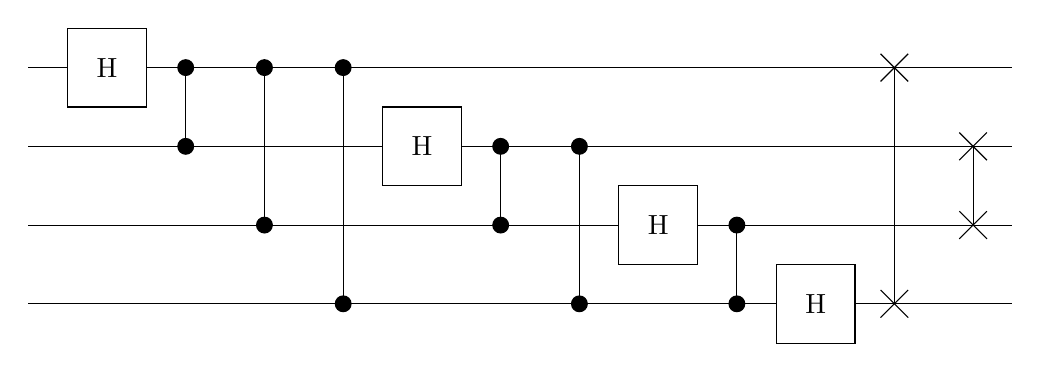
\begin{tikzpicture}[scale=.5]
            \draw (-2, 5) -- (23, 5);
            \draw (-2, 3) -- (23, 3);
            \draw (-2, 1) -- (23, 1);
            \draw (-2, -1) -- (23, -1);

            \draw[fill=white] (-1, 4) -- (-1, 6) -- (1, 6) -- (1,4) -- cycle;
            \node[draw=none] at (0, 5) {H};

            \draw(2, 5) -- (2, 3);
            \draw[fill=black] (2, 5) circle (.2);
            \draw[fill=black] (2, 3) circle (.2);
            \draw(4, 5) -- (4, 1);
            \draw[fill=black] (4, 5) circle (.2);
            \draw[fill=black] (4, 1) circle (.2);
            \draw(6, 5) -- (6, -1);
            \draw[fill=black] (6, 5) circle (.2);
            \draw[fill=black] (6, -1) circle (.2);

            \draw[fill=white] (-1+8, 4-2) -- (-1+8, 6-2) -- (1+8, 6-2) -- (1+8,4-2) -- cycle;
            \node[draw=none] at (8, 5-2) {H};

            \draw(10, 5-2) -- (10, 3-2);
            \draw[fill=black] (10, 5-2) circle (.2);
            \draw[fill=black] (10, 3-2) circle (.2);
            \draw(12, 5-2) -- (12, 3-4);
            \draw[fill=black] (12, 5-2) circle (.2);
            \draw[fill=black] (12, 3-4) circle (.2);

            \draw[fill=white] (-1+8+6, 4-4) -- (-1+8+6, 6-4) -- (1+8+6, 6-4) -- (1+8+6,4-4) -- cycle;
            \node[draw=none] at (8+6, 5-4) {H};

            \draw(16, 5-2-2) -- (16, 3-4);
            \draw[fill=black] (16, 5-2-2) circle (.2);
            \draw[fill=black] (16, 3-4) circle (.2);

            \draw[fill=white] (-1+8+6+4, 4-4-2) -- (-1+8+6+4, 6-4-2) -- (1+8+6+4, 6-4-2) -- (1+8+6+4,4-4-2) -- cycle;
            \node[draw=none] at (8+6+4, 5-4-2) {H};

            \draw (20, 5) -- (20, -1);
            \draw (20 - .35, 5 + .35) -- (20 + .35, 5 - .35);
            \draw (20 - .35, 5 - .35) -- (20 + .35, 5 + .35);
            \draw (20 - .35, -1 + .35) -- (20 + .35, -1 - .35);
            \draw (20 - .35, -1 - .35) -- (20 + .35, -1 + .35);
            \draw (22, 3) -- (22, 1);
            \draw (22 - .35, 3 + .35) -- (22 + .35, 3 - .35);
            \draw (22 - .35, 3 - .35) -- (22 + .35, 3 + .35);
            \draw (22 - .35, 1 + .35) -- (22 + .35, 1 - .35);
            \draw (22 - .35, 1 - .35) -- (22 + .35, 1 + .35);
            \end{tikzpicture}
\]
\pagebreak

\[
       \text{QFT} \, \left(  \sum\limits_{x=0}^{2^N-1} \alpha_x |x\rangle \right) 
       = 
       \frac{1}{\sqrt{2^N}}
        \sum\limits_{x=0}^{2^N-1} \left( 
            \sum\limits_{y=0}^{2^N-1} e^{2 \pi \, i \, x \, y / 2^N} \; \alpha_y
        \right) |x\rangle
    \]
\pagebreak

\[
       \rho \; \rightarrow \; \text{QFT} \; \rho \; \text{QFT}^{\dagger}
    \]
\pagebreak

$\log_2(\text{\#nodes})$
\pagebreak

\[
     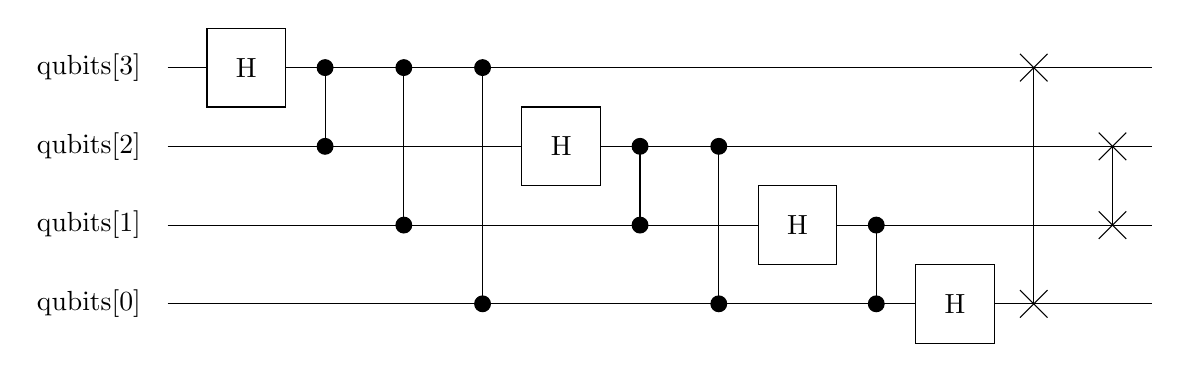
\begin{tikzpicture}[scale=.5]
     \draw (-2, 5) -- (23, 5);    \node[draw=none] at (-4,5) {qubits[3]};
     \draw (-2, 3) -- (23, 3);    \node[draw=none] at (-4,3) {qubits[2]};
     \draw (-2, 1) -- (23, 1);     \node[draw=none] at (-4,1) {qubits[1]};
     \draw (-2, -1) -- (23, -1);  \node[draw=none] at (-4,-1) {qubits[0]};

     \draw[fill=white] (-1, 4) -- (-1, 6) -- (1, 6) -- (1,4) -- cycle;
     \node[draw=none] at (0, 5) {H};

     \draw(2, 5) -- (2, 3);
     \draw[fill=black] (2, 5) circle (.2);
     \draw[fill=black] (2, 3) circle (.2);
     \draw(4, 5) -- (4, 1);
     \draw[fill=black] (4, 5) circle (.2);
     \draw[fill=black] (4, 1) circle (.2);
     \draw(6, 5) -- (6, -1);
     \draw[fill=black] (6, 5) circle (.2);
     \draw[fill=black] (6, -1) circle (.2);

     \draw[fill=white] (-1+8, 4-2) -- (-1+8, 6-2) -- (1+8, 6-2) -- (1+8,4-2) -- cycle;
     \node[draw=none] at (8, 5-2) {H};

     \draw(10, 5-2) -- (10, 3-2);
     \draw[fill=black] (10, 5-2) circle (.2);
     \draw[fill=black] (10, 3-2) circle (.2);
     \draw(12, 5-2) -- (12, 3-4);
     \draw[fill=black] (12, 5-2) circle (.2);
     \draw[fill=black] (12, 3-4) circle (.2);

     \draw[fill=white] (-1+8+6, 4-4) -- (-1+8+6, 6-4) -- (1+8+6, 6-4) -- (1+8+6,4-4) -- cycle;
     \node[draw=none] at (8+6, 5-4) {H};

     \draw(16, 5-2-2) -- (16, 3-4);
     \draw[fill=black] (16, 5-2-2) circle (.2);
     \draw[fill=black] (16, 3-4) circle (.2);

     \draw[fill=white] (-1+8+6+4, 4-4-2) -- (-1+8+6+4, 6-4-2) -- (1+8+6+4, 6-4-2) -- (1+8+6+4,4-4-2) -- cycle;
     \node[draw=none] at (8+6+4, 5-4-2) {H};

     \draw (20, 5) -- (20, -1);
     \draw (20 - .35, 5 + .35) -- (20 + .35, 5 - .35);
     \draw (20 - .35, 5 - .35) -- (20 + .35, 5 + .35);
     \draw (20 - .35, -1 + .35) -- (20 + .35, -1 - .35);
     \draw (20 - .35, -1 - .35) -- (20 + .35, -1 + .35);
     \draw (22, 3) -- (22, 1);
     \draw (22 - .35, 3 + .35) -- (22 + .35, 3 - .35);
     \draw (22 - .35, 3 - .35) -- (22 + .35, 3 + .35);
     \draw (22 - .35, 1 + .35) -- (22 + .35, 1 - .35);
     \draw (22 - .35, 1 - .35) -- (22 + .35, 1 + .35);
     \end{tikzpicture}
\]
\pagebreak

$|x,r\rangle$
\pagebreak

$x$
\pagebreak

$|x_j,r_j\rangle$
\pagebreak

$j\text{th}$
\pagebreak

$n =$
\pagebreak

$N =$
\pagebreak

\[
     (\text{QFT}\otimes 1) \, \left(  \sum\limits_{j=0}^{2^N-1} \alpha_j \, |x_j,r_j\rangle \right) 
     = 
     \frac{1}{\sqrt{2^n}}
      \sum\limits_{j=0}^{2^N-1} \alpha_j \left( 
          \sum\limits_{y=0}^{2^n-1} e^{2 \pi \, i \, x_j \, y / 2^n} \; 
          |y,r_j \rangle
      \right)
  \]
\pagebreak

\[
     \rho \; \rightarrow \; \text{QFT} \; \rho \; \text{QFT}^{\dagger}
  \]
\pagebreak

\[
        \text{state} \to \text{op} \, \text{state} \, \text{op}^\dagger
\]
\pagebreak

\[
        \text{state} \to \text{op} \, \text{state}
\]
\pagebreak

\end{document}
